\chapter{Methods}
Summarizing the key points made in chapter \ref{background}, current deep learning pipelines are not equipped with evaluation methods suitable for out-of-distribution generalization, are largely incapable of reliably learning causally robust features, and are underspecified by the datasets they are trained on. Addressing generalization failure requires mitigating some of these problems. The literature, in broad strokes, tackles this by improving the models' inductive biases, e.g through attention-based mechanisms \cite{attention_generalizability, reverse_attention}, ensembles \cite{divergentnets, endoensemble}, etc, or their support, e.g through data augmentation techniques \cite{polyp_augmentation, cyclegan}. 

This thesis attempts to combine the central ideas behind these methods into one unified deep learning pipeline, intended primarilyto maximize generalizability. Additionally, a novel evaluation procedure and loss function is also introduced. The components of the final pipeline can be summarized as follows:

\begin{itemize}
    \item A custom augmentation strategy, including both conventional augmentation functions and a \gls{gan}-inpainter
    \item A familly of metrics based on a quantity referred to as the \glsfirst{sis} and a corresponding evaluation procedure, intended to capture the consistency of predictors when evaluating across augmented and non-augmented sets
    \item A loss function and training method based on this metric, which optimizes for this notion of consistency, referred to as the \glsfirst{sil}
    \item A model intended to learn more causally robust features through multi-task learning, referred to as InductiveNet
    \item Evaluation using an ensemble of InductiveNets trained according to the above methods
\end{itemize}

By incorporating \gls{sis} into the evaluation pipeline as a surrogate for out-of-distribution performance, the pipeline is endowed with the ability to select the most generalizable predictor from a number of iid-risk-equivalent candidates. Moreover, through optimizing for this metric through the use of \gls{sis}, the model can avoid learning inconsistent features altogether. These are modifications that can be applied to practically any segmentation pipeline, and will as a consequence be tested across a number of different models. 

Most models, however, as discussed in \ref{background}, readily learn spurious features. To mitigate this, a model can be constructed such that it learns more generalizable representations through the use of multi-task learning. This model, namely InductiveNet, acheives this through multi-task learning. Similar to DDANet~\cite{ddanet}, InductiveNet employs a single-encoder dual-decoder architecture, wherein the secondary encoder performs image-reconstruction. This should constrain the latent representations leveraged by the model, and hopefully reduce the likelihood of shortcut learning by the virtue of the fact that the model has to incorporate features that are conducive to both reconstruction and segmentation.

Finally, one can combine several predictor in an ensemble in order to facilitate approximate bayesian inference, which as mentioned in the background has been shown to increase generalizability. 

This section will further detail the implementation of these pipeline modifications, as well as their basis with respect to generalizability theory.

\section{OOD Evaluation}
As discussed at length in the background, distinguishing between generalizable and non-generalziable predictors is not feasible when evaluating only in iid-settings. This is because there is no way of knowing whether the learned features are causally related to the problem, or if they are simply predictive due to some other correlation that is strong in the training domain, but that in practical settings would not have any merit. A \gls{ood}-suitable evaluation procedure therefore requires some way of determining whether the predictor is leveraging non-causal or causal features. Determining what features are causal is, however, an intractable problem. For one, the patterns that neural networks learn are often difficult to identify, and even more difficult to understand intuitively. Though the field of explainable AI has made significant progress in this regard, there simply is not a way to determine the causality of the features learned by \glspl{dnn}. Moreover, establishing  this causality necessitates a complete understanding of the problem the model is trying to reason about in the first place. If this was at all possible, one might as well use the knowledge required to do so to design a classifier using conventional image-analysis. 

Though establishing what is causal is difficult, establishing what \textit{isn't} causal is not all that complicated. To give a concrete example, consider once again the problem of classifying images of cows and camels. Associating the cow class with grass and the camel class with sand is obviously non-causal, since this pattern would not hold if the model for instance is asked to detect cows on Mars or camels on the Moon. To mitigate this, one may simply collect data of cows and camels in differing backgrounds, but such careful curation of datasets is not typically feasible. A better approach is to instead simply augment the data. In particular, one can generate multiple instances of the same sample but with varied backgrounds. Consistency across this augmented set can then be rewarded in order to bias the model towards learning background-invariant features. 

This, of course, applies to more than just modifying backgrounds: the more of these non-causal changes to the input data-  from this point on referred to as perturbations - are accounted for and modelled, the more spurious correlations are excluded from the search, and the more likely the model is to learn the patterns that are actually causal. After all, a pattern can for all intents and purposes be considered causal when it holds when subjected to all forms of perturbations. 

Thus, though rewarding causal behaviour is intractable, punishing non-causal behaviour is not. All that is required to do so is to be able to apply perturbations that highlight the non-causal reasoning the model employs, quantify the model's sensitivity to these perturbations, then minimize this quantity through optimization. The resulting model will then have learned invariance to whatever causally irrelevant information that the perturbation defines. This property of being invariant to perturbations will be referred to as the consistency of the model. 

Thus, this notion of consistency is in effect a surrogate for generalizability; if a model is consistent, it is invariant to non-causal patterns, and if it is invariant to non-causal patterns, it necessarily employs causal patterns. Optimizing for consistency can as a result mitigate both shortcut-learning and underspecification, subject only to the span of the space of perturbations and how well inconsistent behaviour can be quantified. For instance, if the perturbations affect the image such that certain shortcuts are broken, these shortcuts are less likely to be learned. A similar argument can be made for underspecification: if multiple predictors are risk equivalent but nevertheless encode conflicting inductive biases, probing the inductive biases learned by the respective predictors through various perturbations can reveal which are generalizable and which are not.

Naturally, this all presupposes that there is some model that can output all possible perturbations one might desire the model to be invariant to. This is of course not the case. As highlighted by the pervasiveness of adversarial attacks and the relative ineffectiveness of adversarial defences, the perturbations that break DNNs are not necesssarily intuitive and are difficult to analyze in a manner that is conducive to the task of engineering invariance thereto. 

Nevertheless, much stands to be gained if the model learns to be invariant even to a fairly limited space of perturbations. Though generalizability is by no means guaranteed in this case, the odds of learning generalizable features are improved simply because the perturbations limits the types of patterns that a given model can learn. If for instance a white-light endoscopic image is perturbed such that it mimics a narrow-band image, and the model learns to be invariant to this perturbation, predictors that leverage white-light or narrow-band dependent features will no longer be returned from ERM.

This approach, then, requires two components: a perturbation model, and some form of training procedure that imposes invariance to the transformations that the perturbation model employs. To this end, a numeric representation of consistency in the context of segmentation needs to be established.

\section{Segmentation Inconsistency Score}
In the context of segmentation, consistency is the ability of the model to output a reasonably unchanged segmentation when the input data is subjected to some perturbation. Inconsistency, by the same token, is the extent to which the output changes when subjected to a perturbation beyond what should be expected from the transform. One simple approach to express this numerically would simply be to count the number of pixels that change given some perturbation, and normalize this with respect to the total number of pixels, or in other words calculating the intersection over union, also known as the Jaccard Index, across the perturbed and unperturbed segmentations.  However, the ground truth may of course change as a result of the perturbation - if the image is rotated, for example, the segmentation mask should be rotated accordingly. If an image is globally distorted in some way, the segmentation should exhibit the corresponding distortion. If an image is exposed to low-amplitude additive noise, the segmentation should not really be affected at all, and so on. This, of course, all needs to be taken into account. This can be achieved by discounting the proportion of pixels that is expected to change from the overall metric. Formally, this metric, referred to as the \glsfirst{sis} can be expressed as follows:

Let \(Y:=\{y,\hat{y}:=f(x)\}\) be the set consisting of the segmentation labels (masks) and predictions for the unperturbed samples, where \(f(\cdot)\) denotes the model. Let \(\epsilon(\cdot)\) be some perturbation function. Then, let \(A:=\{a:=\epsilon(y),\hat{a}:=f(\epsilon(x))\}\) be the set consisting of segmentation predictions and masks when the input is subjected to a perturbation. Inconsistency can then be defined by:
\begin{equation}
    L_c = \frac{1}{\sum\{y \cup a \cup \hat{y} \cup \hat{a} \}} \sum \{y\ominus\hat{y}\ominus a\ominus\hat{a}\}
\end{equation}
Where \(\ominus \) denotes the symmetric difference, also often referred to as the XOR operator.
This, as mentioned, corresponds to counting the number of pixels that change after the input is subjected to a perturbation - \(\hat{a}\ominus \hat{y}\), but discounting those we expect to change, \(a\ominus y\). 
It should be noted that this metric is minimized not only if the predictions are both correct and consistent with one another, but also if the predictions are both incorrect, so long as whatever change that occurs is consistent with the expected change. This is illustrated in Figure \ref{loss_fn}
\begin{figure}[ht]
    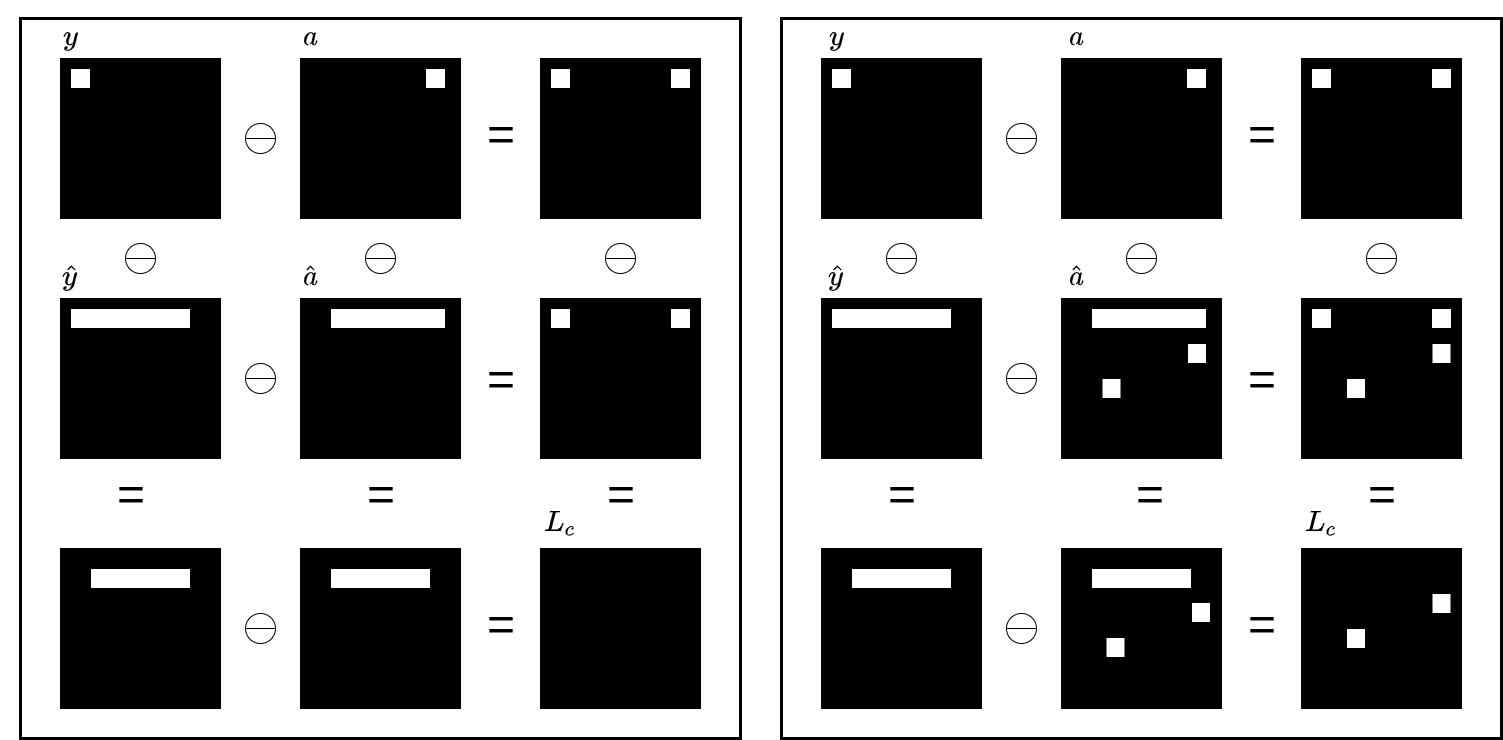
\includegraphics[width=\linewidth]{illustrations/loss_visualisation.drawio.png}
    \caption{Visualisation of \gls{sis} sets, where white is a positive prediction. Note that \gls{sis} is zero regardless of prediction correctness so long as it changes in the expected manner. Note also that the symmetric difference operators are associative. Left shows an instance of consistent and partially incorrect predictions, and right shows an instance of inconsistent and partially correct predictions}
    \label{loss_fn}
\end{figure}  
    
Note, however, that this metric does not presuppose what transformation has occurred. In Figure \ref{loss_fn}, for instance, the change induced by the perturbation may correspond to simply moving the polyp in the image (and replacing the empty space with a believable background), or it may correspond to a rotation by 90 degrees. How this should be analyzed with respect to consistency is up to interpretation - one can argue that a rotation should rotate the incorrect predictions as well, or one can argue that it should only rotate the correct component of the prediction. For simplicity, \gls{sis} is based on the latter interpretation. 

\section{Perturbation Models}
So far, it has been assumed that a perturbation model has been given beforehand. This is of course not the case, and naturally any such model needs to be designed with respect to the domain in question. Rotational invariance makes sense for endoscopic images, for instance, but not for classification of hand-written numbers. Thus, in order to engineer such a model, it is first necessary to establish what invariances are desired for the given task. In the case of polyp-segmentation, it is clear that it is necessary to account for variability in for instance lighting, image-resolution, polyp-size, polyp-shape, polyp-location, camera-quality, color-shifts, blurs, optical distortions, and affine transformations. Thus, a model is required that can (more or less) parametrize this variability. Broadly speaking, these transformations can be categorized as follows:
\begin{itemize}
    \item Pixel-wise variability, which affect only the image, i.e color-shifts, brightness shifts, contrast-shifts,  blurs etc. Practically, this corresponds to changes in lighting conditions, camera motion, dye applications, etc.
    \item Geometric variability, which affect both the image and the segmentation mask by some parametrizable quantity, i.e affine transforms and distortions. Practically, this corresponds to endoscope orientation, optical distortion in the camera, zooming, etc. 
    \item Manifold variablity, which affects both the image and the segmentation mask depending on a learned model of the distribution. Practically, this corresponds to the size, shape and location of the polyps
\end{itemize}
Pixel-wise variability and geometric variability can be modelled fairly trivially through the use of the same transformations typically used in conventional data-augmentation. Manifold-variability, however, is somewhat more difficult, and requires a functional representation of the distribution. \cite{modelbased} and \cite{cyclegan} achieve this through cross-dataset style-transfer, but this of course necessitates multiple datasets. Given only one dataset, a different method must be used. For a classification task, this could for instance be DeepAugment~\cite{deepaugment} or a similar technique. DeepAugment, however, cannot account for the changes in the segmentation mask that should be induced by the augmentations it generates. Consequently, some other generative model wherein the changes in the segmentation mask can be accounted for is required. To this end, a \gls{gan}-inpainter can be used. 

\subsection{GAN-based Polyp Inpainting}
As mentioned in Chapter \ref{background}, the use of GANs and other distributional modelling in the context of generalization is typically restricted to image-to-image translation, and typically involves transforming an image drawn from one distribution such that it is iid with a second distribution. This, though interesting and no doubt useful assuming several such datasets are available, has limited practical use. It is not necessarily always the case that there exists multiple datasets depicting identical problems, and merely translating between modalities does not as mentioned earlier in the thesis ensure generalizability.

A better approach is to try to model the training set distribution directly, then perturb the data in accordance with this model. For segmentation problems, this can be achieved through training a model to fill some predefined region with pixels that correspond to whatever segmentation target the model is meant to learn, in this case polyps, then perturb a given sample by for instance increasing the size of the polyps or adding extra polyps.

To this end, a simple GAN-inpainter was trained. The Generator \(G(\cdot)\) and Discriminator \(D(\cdot)\) were both based on DeepLabV3Plus, and trained using the following loss formulation, where \(L_d\) and \(L_g\) corresponds to the discriminator and generator loss respectively, and \(x\) and \(y\) corresponds to masked selections of the input image and discriminator labels. 
\begin{align}
    L_g &= 0.001 BCE(D(x),y=1) + 0.999 L1(G(x), x) \\
    L_d &= \frac{1}{2}\big[ BCE(D(G(x),y=1)+BCE(D(G(x), y=0)) \big]
\end{align}

This inpainter was then trained using the Adam optimizer and a cosine annealing scheduler with warm restarts. The following hyperparameters were used:

\begin{tabularx}{\linewidth}{@{}XX@{}}
    \toprule
     Hyperparameter & Value \\
     \midrule
     batch\_size & 8 \\
     learning rate & 0.0001 \\
     epochs & 3000 \\
     Scheduler \(T_0\) & 100\\
     Scheduler \(T_{mult}\) & 2 \\
     \bottomrule
\end{tabularx}

Though this implementation is by no means state-of-the-art, it should nevertheless be sufficient for the purpose of augmentation, considering the principal differences between generated and real polyp images are finer textural details and colour balancing, which are affected by the other augmentations anyway. Figure \ref{fig:inpaint} shows some examples of inpaint, alongside real examples.

\begin{figure}
    \centering
    \includegraphics{example-image-b} 
    \caption{GAN-inpainter rexamples}
    \label{fig:inpaint}
\end{figure}

\subsection{Geometric and pixel-wise transformations}
The data was augmented using the \textit{albumentations} ~\cite{albumentations} library for python, which defines a large number of transformations for use in deep learning. To establish which of these augmentations are suitable, one first needs to establish which invariances the model(s) in question should exhibit. \autoref{tab:vanilla_aug} below provides descriptions of the invariances required in the model, and the albumentation function that corresponds to the required transform. 
\begin{table}[ht]
    \centering
\begin{tabularx}{\textwidth}{|X|X|}
    \toprule
    \textbf{Invariance} & \textbf{Albumentation Function}\\
    \midrule
    Perspective &Flip() \newline RandomRotate90()\\
    Resolution and Zoom & RandomCrop() \\
    Image quality &GaussNoise() \newline ImageCompression()\\
    Camera models&OpticalDistortion() \\
    Lighting conditions & ColorJitter() \\
    \bottomrule
\end{tabularx}
    \caption{Overview of albumentation augmentations}
    \label{tab:vanilla_aug}
\end{table}


The parameters for the respective functions where selected as follows: one transformation was considered at a time, then the maximal parameter value(s) that still kept the polyp visible to an untrained eye were identified. Albumentation augmentations simply use this maximum to perform augmentation. The probability of augmentation was set to 0.5 for all the augmentations with the exception of image compression, which always occured since this transform was defined by a range as opposed to a maximal value. To enable scheduling of augmentation severity, the maximal value was scaled in accordance with a temperature parameter. In the end, this temperature was kept at the maximum, as this was the most conducive to increasing consistency. See the appendix for details. 

\begin{figure}
    \centering
    \includegraphics{example-image-a}
    \caption{Sample Augmentations}
    \label{fig:my_label}
\end{figure}

It should also be noted that this set of augmentations, even including the inpainter, is of course not complete - after all, it cannot be, as it would require some way to model any and all changes in the image that do not destroy the possibility of recognizing the polyp. As discussed previously it nevertheless may suffice to model a limited space of these transformations, as it increases the likelihood of learning generalizable features. 


\section{Siamese Consistency Training}

    Similarly to how one can optimize for the Jaccard Index through the Jaccard Loss, so too can one optimize for consistency by using \gls{sis} as a component of a loss function. The perturbation model will then in effect operate as a form of data augmentation, but less stochastic; half of each batch will consist of training samples taken directly from the dataset, with the remaining elements in the batch being these same images, but augmented according to the perturbation model. The model will then in effect be in a siamese configuration, as shown in Figure \ref{fig:consistency_training}
    
    \begin{figure}[ht]
            \centering
            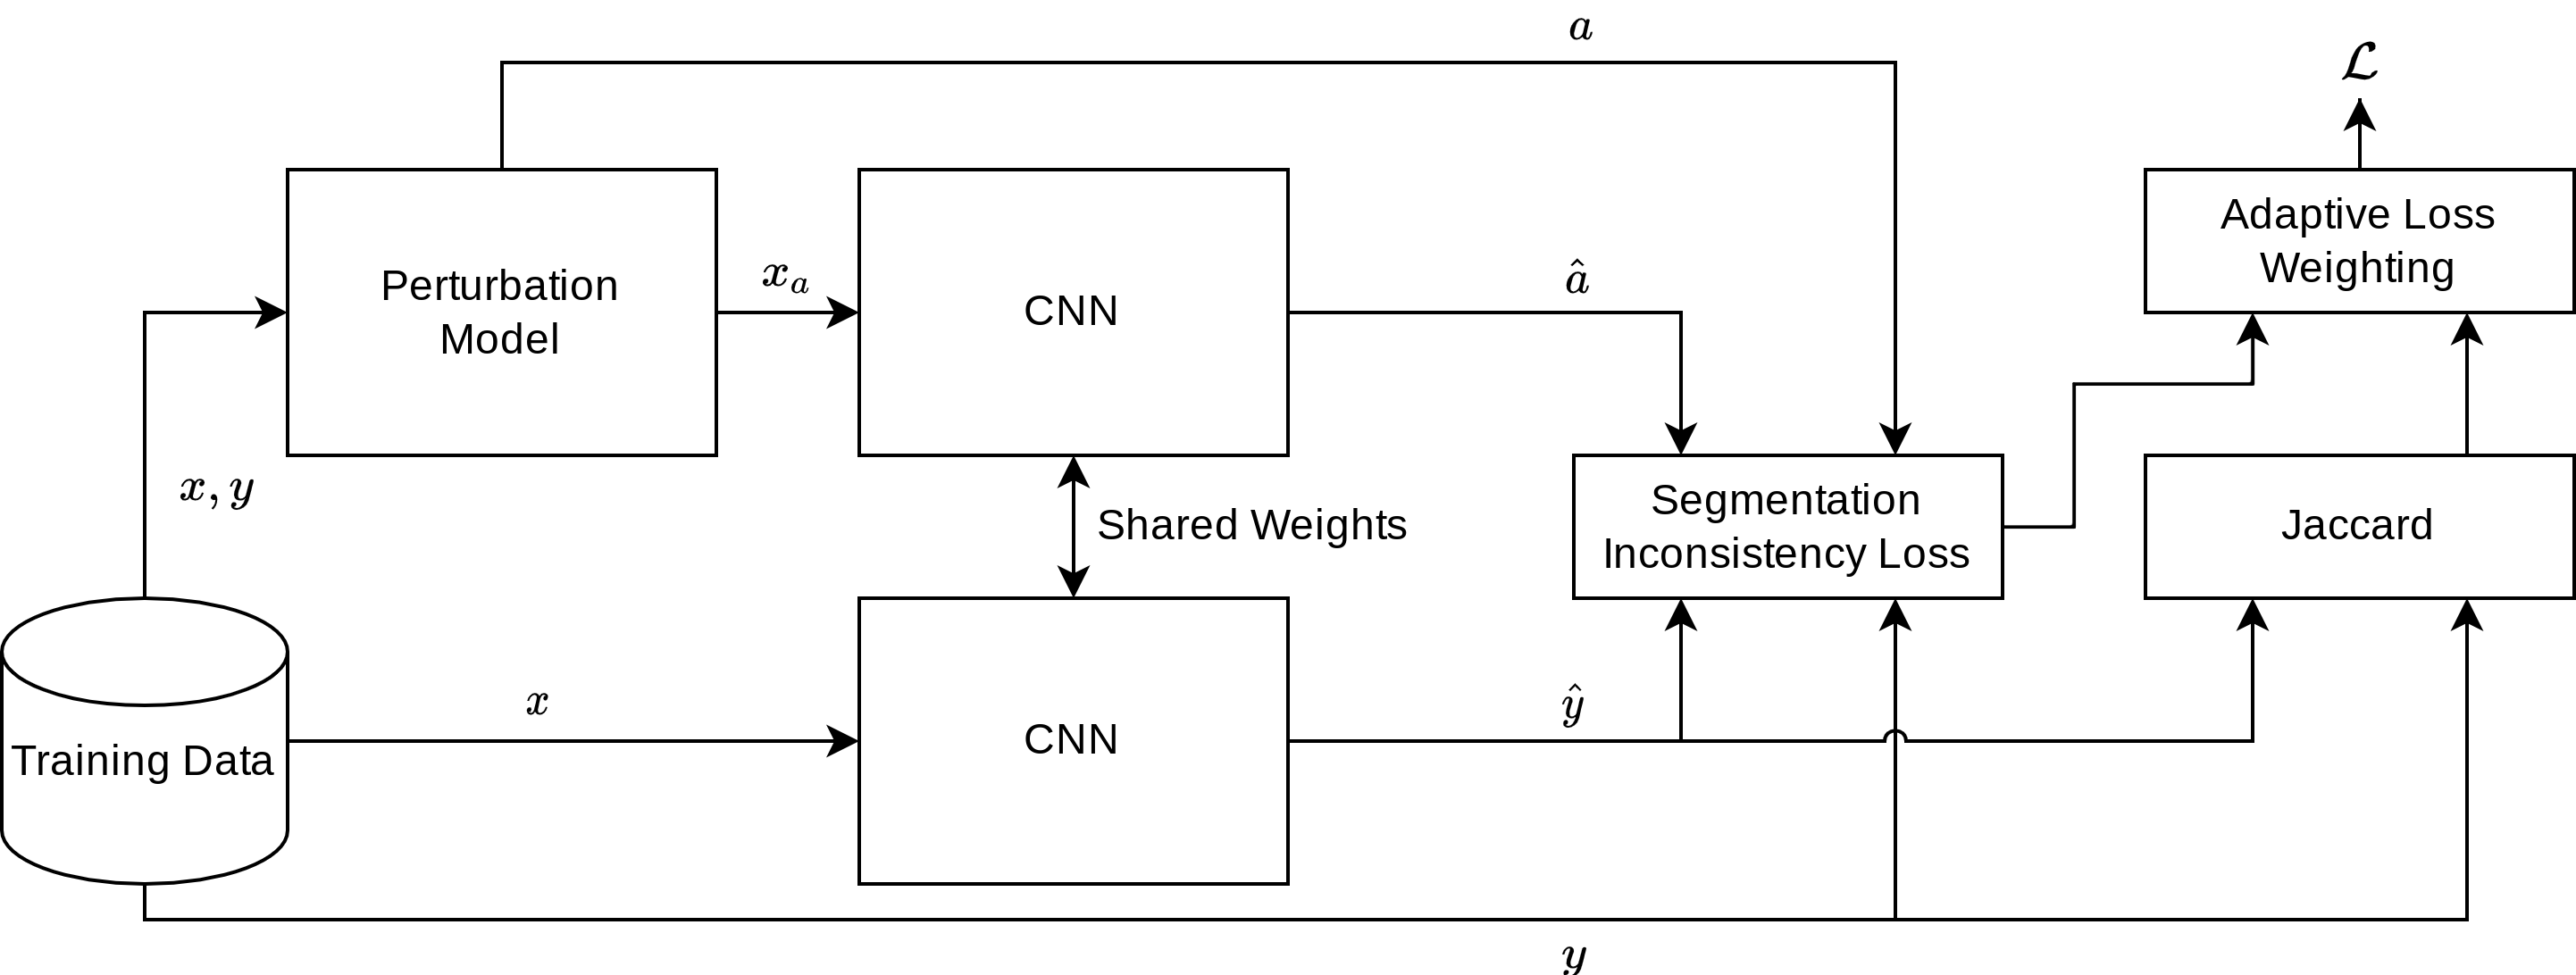
\includegraphics[width=\linewidth]{illustrations/consistency_training.png}
            \caption{Siamese Inconsistency Training}
            \label{fig:consistency_training}
    \end{figure}
    
    Naturally, using \gls{sis} as a loss function on its own is not really useful since it only expresses inconsistency, and is wholly agnostic to whatever object it is trying to segment. Consequently, it has to be combined with a some conventional segmentation loss. A simple way to do this would be to simply add them together and normalize, i.e:
\begin{equation*}
    L(Y, A) = \frac{1}{2} \big[L_{seg}(Y)+L_c(Y,A)\big]
\end{equation*}
Preliminary experiments showed that this, however, exhibited some degree of instability. The model would readily get stuck in local minima where its predictions were indeed consistent, but also consistently predicting artifacts. Examples of this can be found in the appendix. To mitigate this, a better loss function is required. Instead of simply adding the respective losses together, one may weight the individual components adaptively according to the segmentation performance. This way, the model will learn to predict generally correct segmentations early in the training, then start weighing consistency and as a result generalization more and more as the model sees improvements to its segmentation performance:
    \begin{equation}
        L = (1-IoU)\times L_{seg} + IoU \times L_c
    \end{equation}
        If the Jaccard Index (IoU) is used, this is also equivalent to:
    \begin{equation}
        L = {L_{jac}}^2 + (1-L_{jac})L_c
    \end{equation}
Using this formulation, the model will start off trying to learn features that contribute to generally improved segmentation performance, then as segmentation performance improves start principally focusing on learning consistent features. Moreover, if the model starts veering into areas in the loss-landscape that constitute poor segmentation performance, it will self-correct by weighing the segmentation loss more. 

\section{InductiveNet}
Many of the models submitted to the EndoCV2021 challange, and for that matter other models exhibiting high degrees of generalizability, impose certain constraints to the latent representations they are capable of learning, for instance attention-based mechanisms, \cite{attention_generalizability}, decoupling the segmentation process into multiple stages \cite{doubleencdec}, or adding auxilliary tasks \cite{ddanet}. This, in theory, benefits the generalizabiltiy of the model by limiting the search space to areas wherein the learned features better represent the nature of the data the models are attempting to interpret. 

To further investigate the extent to which this affects generalizability, a similar model to DDANet~\cite{ddanet}, albeit fairly simplified, is proposed, wherein a single resnet34 encoder is used in conjunction with two DeepLabv3+ decoders. One decoder performs image reconstruction, while the other performs segmentation. This has the benefit of permitting apples-to-apples comparison with DeepLabV3+, as the segmentation portion of the network is identical to the standard model; the only difference is that the latent representations are strengthened through the reconstruction component. 

\begin{figure}[ht]
    \centering
    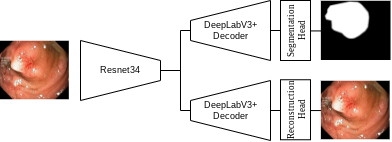
\includegraphics[width=\linewidth]{illustrations/InductiveNet.png}
    \caption{InductiveNet}
    \label{fig:my_label}
\end{figure}
